\PassOptionsToPackage{prologue,dvipsnames}{xcolor}
\documentclass{beamer}
\usepackage[utf8]{inputenc}
\usepackage[english]{babel}
\usepackage{lmodern}

\usepackage{amsthm}
\usepackage{amsmath, amssymb, amsfonts}
\usepackage{mathrsfs}
\usepackage{graphicx}
\graphicspath{ {./Slike/} }
\usepackage{bbm}
\usepackage[dvipsnames]{xcolor}
\usepackage{tikz-cd}
\usepackage{caption}
\usepackage{subcaption}

\newcommand{\A}{\mathcal{A}}
\renewcommand{\AA}{\mathsf{A}}
\newcommand{\B}{\mathcal{B}}
\newcommand{\AB}{\mathsf{B}}
\newcommand{\BB}{\mathscr{B}}
\newcommand{\BBB}{\mathbb{B}}
\renewcommand{\c}{\mathsf{c}}
\newcommand{\E}{\mathsf{E}}
\newcommand{\F}{\mathcal{F}}
\newcommand{\G}{\mathcal{G}}
\renewcommand{\H}{\mathcal{H}}
\newcommand{\M}{\mathcal{M}}
\newcommand{\MM}{\overline{\mathfrak{M}}}
\newcommand{\N}{\mathbb{N}}
\renewcommand{\P}{\mathbb{P}}
\renewcommand{\r}{\mathrm{r}}
\newcommand{\Z}{\mathbb{Z}}
\newcommand{\ZZ}{\mathcal{Z}}

\newcommand{\set}[1]{\left\{#1\right\}}
\newcommand{\oklepaj}[1]{\left(#1\right)}
\newcommand{\oglati}[1]{\left[#1\right]}
\newcommand{\ra}{\rightarrow}
\newcommand{\pika}{\boldsymbol{\cdot}}
\newcommand{\1}{\mathbbm{1}}
\renewcommand{\sp}[1]{\langle #1\rangle}
\newcommand{\ind}{\perp\!\!\!\!\perp}
\renewcommand{\c}{\mathsf{c}}
\newcommand{\5}{\vspace{0.5cm}}
\newcommand{\3}{\vspace{0.3cm}}

\usecolortheme{rose}
\useinnertheme[shadows]{rounded}
\useoutertheme{infolines}
\beamertemplatenavigationsymbolsempty

\usepackage{palatino}
\usefonttheme{serif}

\theoremstyle{definition}
\newtheorem*{form}{Formalities}
\newtheorem{ex}{Example}
\newtheorem{thm}{Theorem}[section]
\newtheorem{prop}[thm]{Proposition}
\newtheorem*{sol}{Solution}
\newtheorem*{dis}{Disclaimer}
\newtheorem{df}[thm]{Definition}
\newtheorem{rem}[thm]{Remark}
\newtheorem{fct}[thm]{Fact}
\newtheorem{lem}[thm]{Lemma}
\newtheorem*{sett}{Setting}
\newtheorem{cor}{Corollary}
\newtheorem*{que}{Question}
\newtheorem*{conj}{Conjecture}
\newtheorem*{rec}{Recipe}
\newtheorem*{goal}{Goal}
\newtheorem*{approach}{Approach}

\begin{document}

% #################################################################################################

\title[Scientific Talk]{Absence of Phase Transitions and Preservation of Gibbs Property Under Renormalization \\\vspace{0.4cm} \small{Scientific Talk}}
\author[Oskar Vavtar]{Oskar Vavtar \\\vspace{0.2cm} \small{Supervisor: Dr.~Evgeny A.~Verbitskiy}}
\date{June 21, 2024}
\institute[LU]{Leiden University, \\ Mathematical Institute}

\begin{frame}
	\titlepage
\end{frame}

\begin{frame}
	\tableofcontents
\end{frame}

% #################################################################################################
% #################################################################################################
% #################################################################################################

\section{Introduction}

% #################################################################################################

\begin{frame}
\frametitle{Preliminaries}
Consider finite alphabet $\A$ and write $\Omega=\A^{\Z^d}$.\pause
\begin{df}[Interactions and Hamiltonians]
\begin{itemize}
	\item[(1)] \textbf{Interaction} is a collection of maps $\Phi=(\Phi_\Lambda)_{\Lambda\Subset\Z^d}$, where
	$$\Phi_\Lambda(\omega) ~=~ \Phi_\Lambda(\omega(x):x\in\Lambda), \quad \omega\in\Omega.$$\pause
	We say $\Phi$ is \textbf{uniformly absolutely convergent} (UAC), $\Phi\in\BB^1(\Omega)$, if
	$$\sup_{x\in\Z^d}\sum_{\Lambda\ni x}\|\Phi_\Lambda\|_\infty ~<~ \infty.$$\pause
	\item[(2)] For $\Phi\in\BB^1(\Omega)$, we consider \textbf{Hamiltonians} $\H=(\H_{\Lambda})_{\Lambda\Subset\Z^d}$,
	$$\H_\Lambda(\omega) ~=~ \sum_{\Delta\cap\Lambda\neq\emptyset}\Phi_\Delta(\omega), \quad \omega\in\Omega.$$
\end{itemize}
\end{df}
\end{frame}

\begin{frame}
\frametitle{Preliminaries}
\begin{df}[Specification and Gibbs measure]
\begin{itemize}
	\item[(1)] For $\Phi\in\BB^1(\Omega)$, \textbf{specification} $\gamma=(\gamma_\Lambda)_{\Lambda\Subset\Z^d}$, is given so that $\gamma_\Lambda(\pika|\pika):\F_\Lambda\times\Omega_{\Lambda^\c}\ra(0,1)$,\pause
	$$\gamma_\Lambda(\omega_\Lambda|\xi_{\Lambda^\c}) ~=~ \frac{1}{\ZZ_\Lambda^\xi}\exp(-\H_\Lambda(\omega_\Lambda\xi_{\Lambda^\c})),$$
	where $\ZZ_\Lambda^\xi$ is the normalization constant.\pause
	\item[(2)] $\mu\in\M_1(\Omega)$ is a \textbf{Gibbs measure} on $\Omega$ consistent with $\Phi$ ($\mu\in\G_\Omega(\Phi)$)\pause~if for each $\Lambda\Subset\Z^d$,
	$$\mu(\omega_\Lambda|\omega_{\Lambda^\c}) ~=~ \gamma_\Lambda^\Phi(\omega_\Lambda|\omega_{\Lambda^\c}) \quad \text{for}~\mu\text{-a.a.}~\omega\in\Omega.$$
\end{itemize}
\end{df}
\end{frame}

\begin{frame}
\frametitle{Preliminaries}
\begin{rem}
\begin{itemize}
	\item[(i)] For $\Lambda\Subset\Z^d$ and $\xi_{\Lambda^\c}$ fixed, $\gamma_{\Lambda}(\pika|\xi_{\Lambda^\c})$ is a probability measure on $\Omega_\Lambda=\A^\Lambda$. This allows for construction of Gibbs measures via weak limits.\pause
	\item[(ii)] While $\G_{\Omega}(\Phi)\neq \emptyset$, we don't necessarily have that $|\G_{\Omega}(\Phi)|=1$. How and when this happens is an important subject in statistical mechanics.
\end{itemize}
\end{rem}
\end{frame}

% #################################################################################################

\begin{frame}
\frametitle{Characterization of Gibbsianity}
\begin{prop}
Let $\mu\in\M_1(\Omega)$. The following are equivalent:\pause
	\begin{itemize}
		\item[(i)] $\mu$ is Gibbs\pause
		\item[(ii)] $\mu$ has the following properties:\pause
		\begin{itemize}
			\item[(a)] \textbf{uniform non-nullness}: $\forall\Lambda\Subset\Z^d$ $\exists \alpha_\Lambda,\beta_\Lambda\in(0,1)$ s.t.
			$$\alpha_\Lambda ~\leq~ \mu_\Lambda(\omega_\Lambda|\xi_{\Lambda^\c}) ~\leq~ \beta_\Lambda, \quad \forall \omega,\xi\in\Omega,$$\pause
			\item[(b)] \textbf{quasilocality}: writing $\BBB_n=[-n,n]^d\cap\Z^d$, $\forall \Lambda\Subset\Z^d$,
			$$\sup_{\omega}\sup_{\xi,\zeta}|\mu(\omega_\Lambda|\omega_{\BBB_n\setminus\Lambda}\xi_{\BBB_n^\c\setminus\Lambda})-\mu(\omega_\Lambda|\omega_{\BBB_n\setminus\Lambda}\zeta_{\BBB_n^\c\setminus\Lambda})| ~\ra~ 0.$$ 
		\end{itemize}
	\end{itemize}
\end{prop}
\end{frame}

% #################################################################################################

\begin{frame}
\frametitle{Source of all problems: Renormalization Group}
We want to consider a probability kernel $T$ from $\Omega$ to another space $\Omega'$. \\\vspace{0.5cm}\pause
\textcolor{teal}{\textbf{Example:}} decimation 
\begin{center}
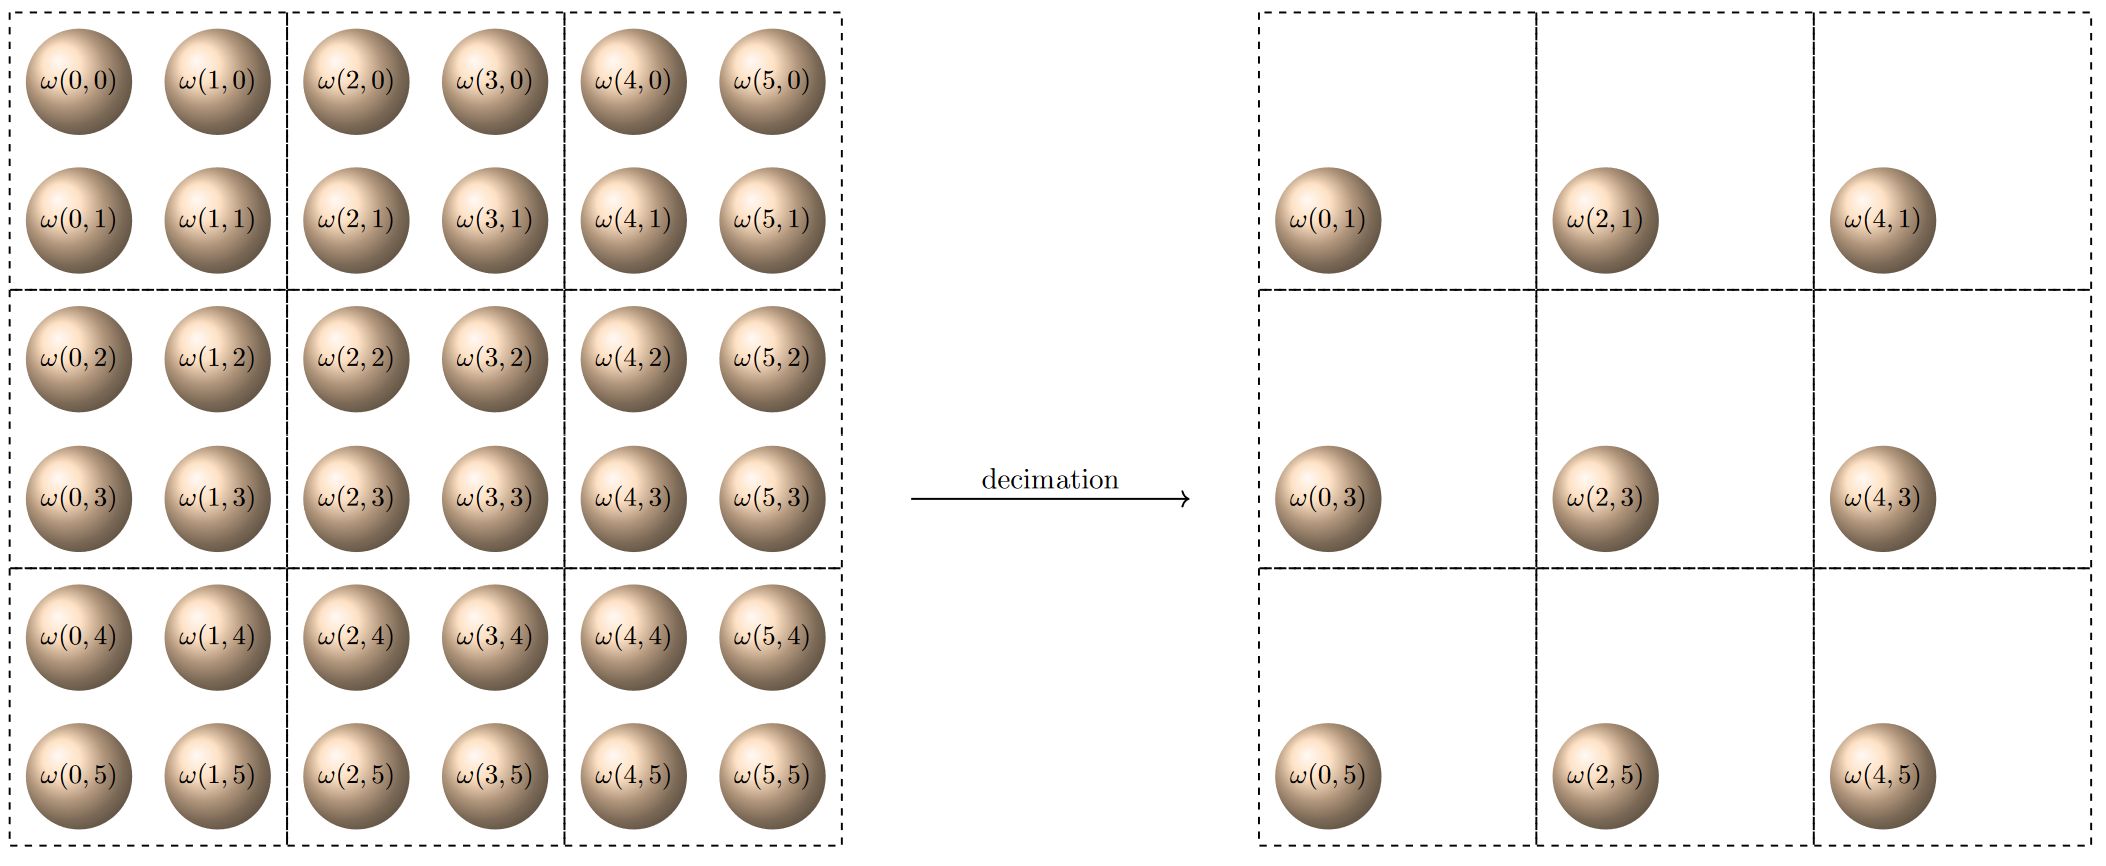
\includegraphics[scale=0.4]{decimation}
\end{center}
\end{frame}

\begin{frame}
\frametitle{Source of all problems: Renormalization Group}
\textcolor{red}{\textbf{Question:}} If $\omega\sim\mu$, with $\mu$ Gibbs (consistent with $\H$), what about the law of $\omega'$.\\\vspace{0.5cm}\pause
In finite volume:\\
\begin{center}
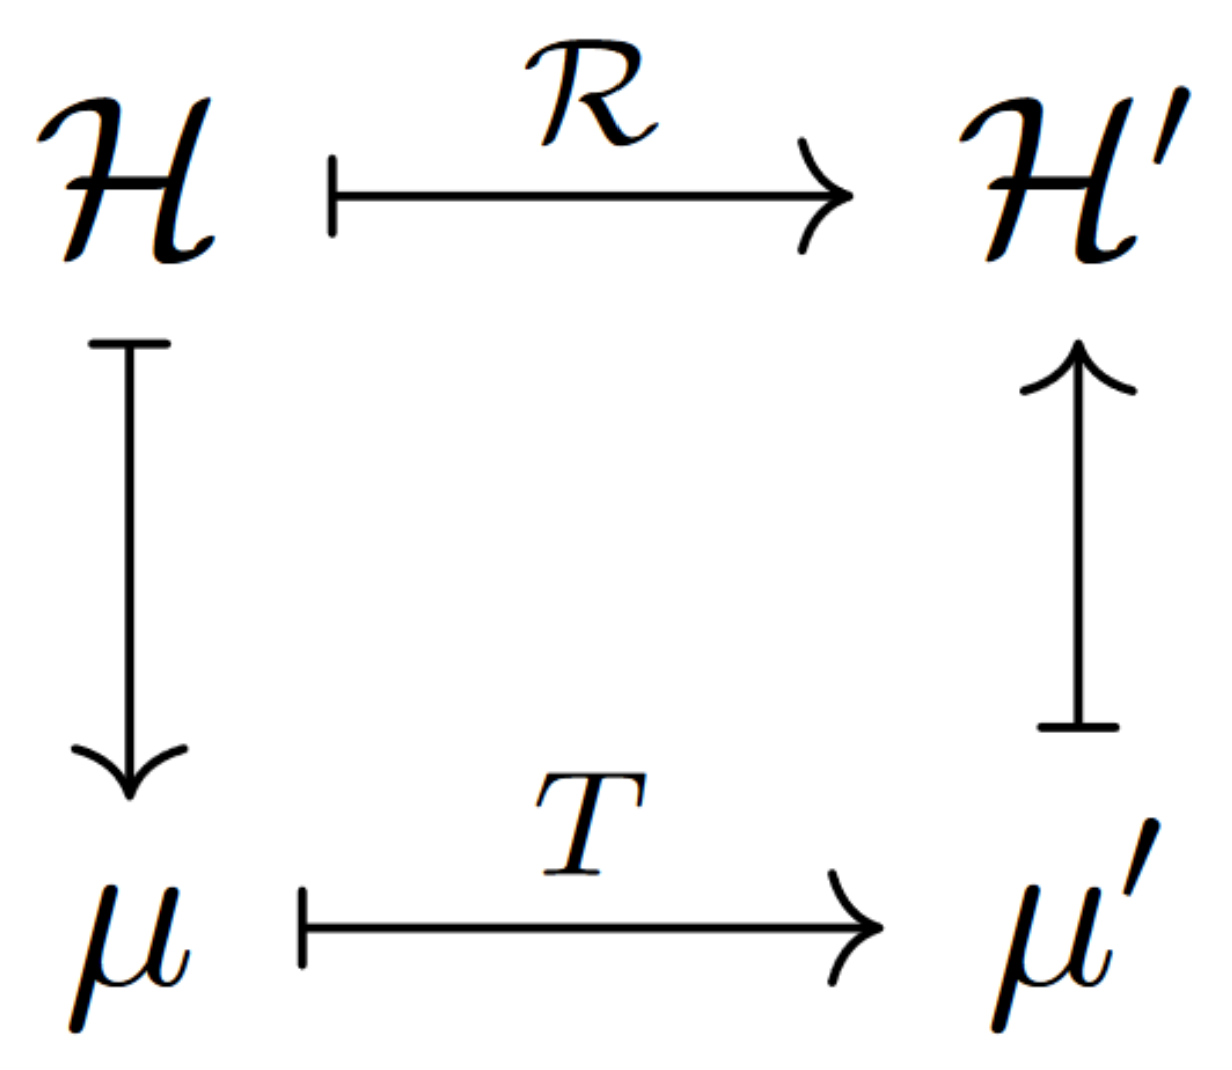
\includegraphics[width=0.2\textwidth]{diagram}
\end{center}\pause
\textcolor{red}{\textbf{Problem:}} In finite volume, $\mu'$ might not be Gibbsian at all, so we cannot speak of $\H'$,\footnote{Fails to be consistent with any quasilocal specification.} $\mathcal{R}$ doesn't make sense.
\end{frame}

% #################################################################################################
% #################################################################################################
% #################################################################################################

\section{Fuzzy Gibbs framework}

% #################################################################################################

\begin{frame}
\frametitle{Fuzzy Gibbs measures}
Consider $\Omega=\A^{\Z^d}$, with $\A$ finite, as before. \\\vspace{0.5cm}\pause
Let $\B$ be another alphabet, with $|\B|\leq|\A|$. Write $\Sigma=\B^{\Z^d}$. \\\vspace{0.5cm}\pause
We consider a surjection $\pi:\A\ra\B$, which we call a \textbf{fuzzy map}.\footnote{$\pi$ induces a surjection $\Omega\ra\Sigma$ which we denote by the same letter}\pause
\begin{df}
A fuzzy Gibbs measure $\nu$ on $\Sigma$ is defined as
$$\nu ~=~ \mu\circ\pi^{-1},$$
where $\mu$ is some Gibbs measure on $\Omega$.
\end{df}\vspace{0.2cm}\pause
\textcolor{red}{\textbf{Question:}} when is $\nu$ Gibbsian?
\end{frame}

% #################################################################################################

\begin{frame}
\frametitle{Hidden phase transitions}
We can partition $\Omega$ w.r.t.~$\pi$ as follows:\\\vspace{0.3cm}\pause
pick $\sigma\in\Sigma$ and define
$$\Omega_\sigma ~=~ \pi^{-1}(\sigma);$$
we call sets $\set{\Omega_\sigma:\sigma\in\Sigma}$ \textbf{fibres}.\pause
\begin{df}[Hidden phase transition]
We say that a \textbf{hidden phase transition} occurs on $\Omega_\sigma$ if
$$|\G_{\Omega_\sigma}(\Phi)| ~>~ 1.$$\pause
If $|\G_{\Omega_\sigma}(\Phi)|=1$ for all $\sigma\in\Sigma$, we talk about \textbf{absence of hidden phase transitions}.

\end{df}
\end{frame}

\begin{frame}
\frametitle{Hidden phase transitions}
\begin{prop}[Sufficient condition]
In the absence of hidden phase transitions, $\nu=\mu\circ\pi^{-1}$ is Gibbsian.
\end{prop}\vspace{0.3cm}\pause
The following conjecture (stated informally here) was established by van Enter, Fern\'andez and Sokal:\pause
\begin{conj}[van Enter-Fern\'andez-Sokal hypothesis, \cite{EFS},\cite{Ber}]
The fuzzy Gibbs measure is not Gibbsian \textit{if and only if}\pause
\begin{itemize}
	\item[(i)] $\exists\sigma\in\Sigma:|\G_{\Omega_\sigma}(\Phi)|>1$, i.e., a hidden phase transition occurs, and\pause
	\item[(ii)] one can pick different phases of $\G_{\Omega_\sigma}(\Phi)$ by varying boundary conditions.
\end{itemize}
\end{conj}
\end{frame}

% #################################################################################################

\begin{frame}
\frametitle{Construction of conditional measures}
\textcolor{teal}{\textbf{Goal:}} construct distribution of $\omega$, conditional on $\pi(\omega)=\sigma$\pause
\begin{df}
Given $B\subseteq\Sigma$ measurable with $\nu(B)>0$, define
$$\mu^B ~=~ \mu(\pika|\pi^{-1}(B)).$$
\end{df}\pause
One can consider a net of conditional measures $\mu^B$ (on $\Omega$), indexed with pairs $(V,B)$, where $V$ is an open neighbourhood of $\sigma$ and $B\subseteq V:\nu(B)>0$. \\\vspace{0.5cm}\pause
Write $\MM_\sigma$ for accumulation points of the above net, as open neighbourhoods ($V$) ``approach'' $\sigma$.
\end{frame}

\begin{frame}
\frametitle{Tjur points}
\begin{df}
If $|\MM_\sigma|=1$ for a given $\sigma\in\Sigma$, denote by $\mu^\sigma$ the only member of $\MM_\sigma$, the limit of the corresponding net. In this case, we say that $\sigma$ is a \textbf{Tjur point}.\pause
\end{df}\vspace{0.3cm}
One can restate the previously presented conjecture as follows:\pause
\begin{conj}[van Enter-Fern\'andez-Sokal hypothesis, \cite{Ber}]
The fuzzy Gibbs measure is Gibbsian \textit{if and only if} $|\MM_\sigma|=1$ for all $\sigma\in\Sigma$, i.e., all points are Tjur.
\end{conj}\vspace{0.3cm}\pause
\begin{prop}[Berghout, Verbitskiy, \cite{Ber}]
Direction $(\Leftarrow)$ holds.
\end{prop}
\end{frame}

\begin{frame}
\frametitle{Tjur points: sufficient condition revisited}
\begin{prop}
$\MM_\sigma\neq 0$, each member is a probability measure supported on $\Omega_\sigma$. If $\mu\in\G_\Omega(\Phi)$, then 
$$\MM_\sigma ~\subseteq~ \G_{\Omega_\sigma}(\Phi).$$
\end{prop}\vspace{0.2cm}\pause
\begin{cor}
Absence of phase transitions implies Gibbsianity of $\nu=\mu\circ\pi^{-1}$.
\end{cor}\vspace*{0.2cm}\pause
\begin{rem}
By demonstrating the absence of phase transitions, we not only obtain Gibbsianity of the fuzzy Gibbs measure, but also verify that the example doesn't contradict the unproven direction of the van Enter-Fern\'andez-Sokal hypothesis.
\end{rem}
\end{frame}

% #################################################################################################
% #################################################################################################
% #################################################################################################

\section{Fuzzy Potts model}

% #################################################################################################

\begin{frame}
\frametitle{Classical Potts model}
Write $\E^d$ for the (nearest-neighbour) edge set of $\Z^d$ and
$$\E_\Lambda=\set{\sp{x,y}\in\E^d:x,y\in\Lambda}, \quad \partial\E_\Lambda=\set{\sp{x,y}\in\E^d:x\in\Lambda,y\notin\Lambda}.$$\pause
\begin{df}[Interaction of Potts model]
The interaction of $q$-state Potts model $\Phi_{\beta,q}$ is given by
$$\Phi_{\Lambda;\beta,q}(\omega) ~=~ \begin{cases}
2\1_{\set{\omega(x)\neq\omega(y)}}-1, ~& \Lambda=\set{x,y}:x\sim y, \\
0, ~&\text{otherwise}.
\end{cases}$$
\end{df}\pause
Hamiltonians are thus given by
$$\H_{\Lambda;\beta,q}(\omega) ~=~ \beta\sum_{\sp{x,y}\in\E_\Lambda\cup\partial\E_\Lambda}(2\1_{\set{\omega(x)\neq\omega(y)}}-1).$$
\end{frame}

\begin{frame}
\frametitle{Classical Potts model: phase transition}
Write $\Omega=\set{1,\ldots,q}^{\Z^d}$.\vspace{0.3cm}
\begin{thm}
For each $q\geq 2$ and $d\geq 2$, there exists $\beta_c(d,q)\in(0,\infty)$, such that \pause
\begin{itemize}
	\item[(i)] for $\beta<\beta_c(d,q)$, $|\G_{\Omega}(\Phi_{\beta,q})|=1$,\pause
	\item[(ii)] for $\beta>\beta_c(d,q)$, $\G_{\Omega}(\Phi_{\beta,q})$ contains $q$ distinct mutually singular measures .
\end{itemize}
\end{thm}\pause\vspace{0.3cm}
Mutually singular measures in (ii) are precisely measures $\mu_{\beta,q}^{\Z^d,1},\ldots,\mu_{\beta,q}^{\Z^d,q}$, corresponding to constant boundary conditions $\mathsf{1},\ldots,\mathsf{q}$.
\end{frame}

% #################################################################################################

\begin{frame}
\frametitle{Fuzzy Potts model}
Let $1<s<q$ and $\r=(r_1,\ldots,r_s)$, such that $r_1+\ldots+r_s=q$.\pause
\begin{df}
Fuzzy Potts map $\pi_\r:\set{1,\ldots,q}\ra\set{1,\ldots,s}$ is given by
$$\pi_\r(a) ~=~ \begin{cases}
1: ~&1\leq a\leq r_1, \\
2: ~&r_1+1<a\leq r_1+r_2, \\
\ldots \\
n: ~& r_1+\ldots+r_{n-1}<a\leq r_1+\ldots r_n, \\
\ldots \\
s: ~& r_1+\ldots+r_{s-1}<a\leq q.
\end{cases}$$\pause
Fuzzy Gibbs measure corresponding to $\mu_{\beta,q}^{\Z^d,\xi}$ is given by
$$\nu_{\beta,q}^{\Z^d,\xi} ~=~ \mu_{\beta,q}^{\Z^d,\xi}\circ\pi_{\r}^{-1}.$$
\end{df}
\end{frame}

\begin{frame}
Write $r^*=\min(\set{r_1,\ldots,r_s}\cap\N_{\geq 2})$
\frametitle{Fuzzy Potts model: Gibbsianity}
\begin{thm}[H\"aggstr\"om, \cite{Hag}]
Let $d\geq 2$, $q\geq 3$ and $\xi\in\set{\emptyset,\mathsf{1},\ldots,\mathsf{q}}$; consider fuzzy Potts measure $\mu_{\beta,q}^{\Z^d,\xi}$.\pause
\begin{itemize}
	\item[(i)] For each $\beta<\beta_c(d,r^*)$, $\nu_{\beta,q}^{\Z^d,\xi}$ is a Gibbs measure.\pause
	\item[(ii)] For each $\beta>\frac{1}{2}\log\frac{1+(r^*-1)p_c(d)}{1-p_c(d)}$, $\nu_{\beta,q}^{\Z^d,\xi}$ is \textit{not} a Gibbs measure.\footnote{$p_c(d)$ = critical probability for Bernoulli percolation on $\Z^d$}
\end{itemize}
\end{thm}\vspace{0.3cm}\pause
\textcolor{teal}{\textbf{Goal:}} provide an alternative proof of (i), using absence of hidden phase transitions.
\end{frame}

% #################################################################################################

\begin{frame}
\frametitle{Idea of alternative proof}
\textcolor{teal}{\textbf{Want to show:}} for each $\sigma\in\set{1,\ldots,s}^{\Z^d}$, $|\G_{\Omega_\sigma}(\Phi_{\beta,q})|=1$. \\\vspace{0.5cm}\pause
\textcolor{orange}{\textbf{Notice:}} 
$$\Omega_\sigma ~=~ \prod_{x\in\Z^d}\pi^{-1}(\sigma(x));$$\pause
write, for $j=1,\ldots,s$, 
$$\AA_j ~=~ \pi^{-1}(j) ~=~ \set{r_1+\ldots+r_{j-1}+1,\ldots,r_1+\ldots+r_j}$$\pause
and
$$U_j ~=~ \set{x\in\Z^d:\sigma(x)=j}.$$\pause
Then,
$$\Omega_\sigma ~=~ \prod_{x\in\Z^d}\begin{cases}
\AA_1, ~&x\in U_1, \\
\ldots \\
\AA_s, ~&x\in U_s
\end{cases} ~=:~ \bigotimes_{j=1}^s \AA_j^{U_j}.$$
\end{frame}

\begin{frame}
\frametitle{Idea of alternative proof}
It is enough to show that:\vspace{0.3cm}\pause
\begin{itemize}
	\item[(i)] If $\beta$ is such that 
	$$|\G_{\AA_j^{\Z^d}}(\Phi_{\beta,|\AA_j|})| ~=~ 1, \quad \forall j=1,\ldots,s,$$\pause
	then
	$$|\G_{\AA_j^{U_j}}(\Phi_{\beta,|\AA_j|})| ~=~ 1, \quad \forall j=1,\ldots,s.$$\pause
	\item[(ii)] If 
	$$|\G_{\AA_j^{U_j}}(\Phi_{\beta,|\AA_j|})| ~=~ 1, \quad \forall j=1,\ldots,s,$$\pause
	then
	$$|\G_{\otimes_j\AA_j^{U_j}}(\Phi_{\beta,q})| ~=~ 1.$$
\end{itemize}
\end{frame}

\begin{frame}
\frametitle{Idea of alternative proof}
\textcolor{orange}{\textbf{Clear:}} enough to show above for $s=2$, induction takes care of the rest. Thus sufficient to prove:\pause
\begin{prop}[Part I]
Let $U\subset\Z^d$ and $q\in\N_{\geq 2}$. For $\beta<\beta_c(d,q)$,
$$|\G_{\set{1,\ldots,q}^U}(\Phi_{\beta,q})| ~=~ 1.$$
\end{prop}\pause
\begin{prop}[Part II]
Let $\Z^d=U\sqcup V$ and $\AA\cap\AB=\emptyset$. If $\beta$ is such that
$$|\G_{\AA^U}(\Phi_{\beta,|\AA|})| ~=~ |\G_{\AB^V}(\Phi_{\beta,|\AB|})| ~=~ 1,$$
then
$$|\G_{\AA^U\otimes\AB^V}(\Phi_{\beta,|\AA|+|\AB|})| ~=~ 1.$$
\end{prop}
\end{frame}

% #################################################################################################
% #################################################################################################
% #################################################################################################

\section{Spin-flip dynamics}

% #################################################################################################

\begin{frame}
\frametitle{Spin-flip dynamics: general model}
\textcolor{teal}{\textbf{Idea:}} Pick initial configuration $\omega_0\in\set{-1,+1}^{\Z^d}$ according to some Gibbs measure and randomly flip spins as time runs. \\\vspace{0.5cm}\pause
\textcolor{orange}{\textbf{Question:}} Having obtained $(\omega_t)_{t\geq 0}$, when is $\mathrm{Law}(\omega_t)$ Gibbsian?
\end{frame}

\begin{frame}
\frametitle{Spin-flip dynamics: general model}
Let $\Omega_*=\set{-1,+1}^{\Z^d}$.\\\vspace{0.5cm}\pause
Pick $\mu\in\G_{\Omega_*}$ and draw $\omega_0\sim\mu$. \\\vspace{0.5cm}\pause
Obtain $(\omega_t)_{t\geq 0}$ by flipping random spin at random times;\pause~dynamics are induced by rates $c(x,\omega)$,\pause~which are \textit{translation invariant} in the second coordinate\pause~and depend on the second coordinate through a finite set, admitting an uniform bound on its diameter. \\\pause\vspace*{0.5cm}
This induces a semigroup $(S(t))_{t\geq 0}$ acting on $\M_1(\Omega_*)$, so that
$$\mu S(t) ~=~ \mathrm{Law}(\omega_t).$$
\end{frame}

% #################################################################################################

\begin{frame}
\frametitle{High-temperature dynamics model}
We now assume that $c(x,\omega)$ does no longer depend on neither $x$ nor $\omega$. \\\vspace*{0.5cm}\pause
In other words: each $(\omega_t(x))_{t\geq 0}$ evolves independently, is flipped according to an exponential rate $c>0$.\\\vspace{0.5cm}\pause
\textcolor{teal}{\textbf{Tranditional approach:}} instead of $\mathrm{Law}(\omega_t)$, study
$$\hat{\mu}_t ~:=~ \mathrm{Law}(\omega_0,\omega_t).$$\pause
\textit{If} $\hat{\mu}_t$ is Gibbsian on $\Omega=\Omega_*\times\Omega_*$, consistent with Hamiltonian $\hat{\H}^{(t)}$, one can show that $\mu S(t)$ is Gibbsian\pause~by verifying that
$$|\G_{\Omega_*}(\hat{\H}^{(t)}(\pika,\eta))| ~=~ 1, \quad \forall \eta\in\Omega_*.$$
\end{frame}

% #################################################################################################

\begin{frame}
\frametitle{Two theorems}
We will say that $\Phi\in\BB^1(\Phi)$ (or its associated Hamiltonian) is \textit{high-temperature} if
$$\sup_{x\in\Z^d}\sum_{\Lambda\ni x}(|\Lambda|-1)\sup_{\omega,\tilde{\omega}}|\Phi_\Lambda(\omega)-\Phi_\Lambda(\tilde{\omega})| ~<~ 2.$$\pause
$\Phi$ being high-temperature implies $|\G(\Phi)|=1$ (via Dobrushin's Uniqueness Condition). \pause
\begin{thm}[\cite{EFHR}]
Assuming dynamics as above and $\mu$ either high-temperature or infinite-temperature (i.i.d.), then $\mu S(t)$ is Gibbsian for all $t\geq 0$.
\end{thm}
\end{frame}

\begin{frame}
\frametitle{Two theorems}
Write $\mu_{\beta,h}$ for some Gibbs measure for Ising model, i.e., consistent with 
$$\H_\Lambda(\omega) ~=~ -\beta\!\!\sum_{\sp{x,y}\in\E_\Lambda\cup\partial\E_\Lambda}\!\!\!\omega(x)\omega(y) - h\sum_{x\in\Lambda}\omega(x),$$
with $\beta>0$ inverse temperature, $h\in\mathbb{R}$ external magnetic field.\pause
\begin{thm}[\cite{EFHR}]
Let $\mu_{\beta,h}$ be as above for $\beta\gg\beta_c(d)$.\pause
\begin{itemize}
	\item[(i)] There exists $t_0=t_0(\beta,h)$, so that $\mu_{\beta,h}S(t)$ is Gibbsian for $t\leq t_0$.\pause
	\item[(ii)] Moreover, if $h>0$ then there exists $t_1=t_1(\beta,h)$, so that $\mu_{\beta,h}S(t)$ is Gibbsian for $t\geq t_1$.
\end{itemize}
\end{thm}
\end{frame}

% #################################################################################################

\begin{frame}
\frametitle{High-temperature dynamics as a fuzzy model}
We notice that since each $(\omega_t(x))_{t\geq 0}$ evolves independently, being flipped at exponential rate $c>0$, \pause
$$[\mu S(t)](\omega_t(x)=1) = \mu(\omega_0(x)=1)\P\!\oklepaj{\substack{\text{even flips}\\\text{until}~t}}+\mu(\omega_0(x)=-1)\P\!\oklepaj{\substack{\text{odd flips}\\\text{until}~t}},$$\pause
where probabilities of even/odd flips are given by
$$\frac{1\pm e^{-2tc}}{2}.$$\pause
Writing $\kappa(t)=\frac{1}{2}(1-e^{-2tc})$, we obtain
$$[\mu S(t)](\omega_t(x)=1) ~=~ \mu(\omega_0(x)=1)(1-\kappa(t))+\mu(\omega_0(x)=-1)\kappa(t).$$
\end{frame}

\begin{frame}
\frametitle{High-temperature dynamics as a fuzzy model}
Fix $\kappa\in[0,1]$ and let $X\sim\mu$.\\\vspace{0.5cm}\pause
Define $\Omega_*$-valued r.v.~$Y^\kappa$, so that $(Y^\kappa(x))_{x\in\Z^d}$ are i.i.d.~with
$$Y^\kappa(x) ~=~ \begin{cases}
1, ~&\text{with probability}~1-\kappa,\\
-1, ~&\text{with probability}~\kappa,
\end{cases}$$
and denote its law by $\rho^\kappa$. \\\vspace{0.5cm}\pause
Define now $Z^\kappa=X\cdot Y^\kappa$ and denote its law by $\nu^\kappa$. \\\vspace{0.5cm}\pause
Clearly
$$\nu^\kappa(Z^\kappa(x)=1) ~=~ \mu(X(x)=1)(1-\kappa) + \mu(X(x)=-1)\kappa.$$
\end{frame}

\begin{frame}
\frametitle{High-temperature dynamics as a fuzzy model}
Define
\begin{align*}
\pi:\Omega&\ra\Omega_*\\
(\omega_\mathsf{c},\omega_\mathsf{d})&\mapsto\omega_\mathsf{c}\cdot\omega_\mathsf{d}
\end{align*}\pause
It is clear that
$$\nu^\kappa ~=~ (\mu\otimes\rho^\kappa)\circ\pi^{-1}.$$\\\vspace{0.2cm}\pause
Both $\mu$, $\rho^{\kappa}$ are Gibbsian\pause~$\Rightarrow$ $\mu\otimes\rho^{\kappa}$ is Gibbsian\pause~$\Rightarrow$ $\nu^\kappa$ is fuzzy Gibbs.\\\vspace*{0.5cm}\pause
Moreover, choosing $\kappa(t)$ (as defined before), we obtain precisely
$$\nu^{\kappa(t)} ~=~ \mu S(t).$$
\end{frame}

% #################################################################################################

\begin{frame}
\frametitle{Alternative proof strategy}
To verify Gibbsianity of $\mu S(t)=\nu^{\kappa(t)}$, it is enough to show that for each $\sigma\in\Omega_*$, 
$$|\G_{\Omega_\sigma}(\H^{\kappa(t)})| ~=~ 1,$$
where $\H^{\kappa(t)}$ is a Hamiltonian with which $\mu\otimes\rho^{\kappa(t)}$ is consistent. \\\vspace{0.5cm}\pause
One notices that in fact
$$\Omega_\sigma ~=~ \set{\!\oklepaj{\omega,\frac{\sigma}{\omega}}:\omega\in\Omega_*} ~=~ \set{(\omega,\omega\sigma):\omega\in\Omega_*}.$$\\\vspace{0.2cm}\pause
Thus sufficient to show that for each $\sigma\in\Omega_*$,
$$|\G_{\Omega_*}(\H^{\kappa(t)}(\pika,\pika\sigma))| ~=~ 1.$$
\end{frame}

\begin{frame}
\frametitle{Alternative proof strategy}
\textcolor{teal}{\textbf{Main trick:}} Given any fixed $\sigma\in\Omega_*$,
$$\H^{\kappa(t)}(\pika,\pika\sigma)-\hat{\H}^{(t)}(\pika,\sigma)$$
corresponds to a single-site interaction\pause~$\Rightarrow$ one is high-temperature iff the other is.
\end{frame}

% #################################################################################################
% #################################################################################################
% #################################################################################################

\section*{~}

\begin{frame}
	\begin{thebibliography}{++}

\bibitem[Ber20]{Ber} S.~Berghout. \textit{Gibbs Processes and Applications}. Ph.D.~thesis. Leiden University, 2020.

\bibitem[vEFdHR02]{EFHR} A.C.D.~van Enter, R.~Fern\'andez, F.~den Hollander, F.~Redig. \textit{Possible Loss and Recovery of Gibbsianness During the Stochastic Evolution of Gibbs Measures}. Commun.~Math.~Phys.~226 (2002), 101-130.

\bibitem[vEFS93]{EFS} A.C.D.~van Enter, R.~Fern\'andez, A.D.~Sokal. \textit{Regularity properties and pathologies of position-space renormalization-group transformations: Scope and limitations of Gibbsian theory}. J.~Statist.~Phys.~72 (1993), no.~5-6, 879-1167.

\bibitem[H\"ag03]{Hag} O.~H\"aggstr\"om. \textit{Is the fuzzy Potts model Gibbsian?} Ann.~I.~H.~Poincar\'e 39 (2003), no.~5, 891-917.

	\end{thebibliography}
\end{frame}

% #################################################################################################

\end{document}
